\documentclass[final,hyperref={pdfpagelabels=false},aspectratio=169,t]{beamer}
\mode<presentation> {
  \usecolortheme{rose}
  \setbeamertemplate{footline}[page number] 
  \setbeamertemplate{navigation symbols}{} 
  \usefonttheme{professionalfonts}}

\usepackage{graphicx} % Allows including images
\usepackage{booktabs} % Allows the use of \toprule, \midrule and \bottomrule in tables

\usepackage{geometry}
\usepackage{xspace}

\usepackage[utf8]{inputenc}
\usepackage{default}
\usepackage{amsmath}
\usepackage{amsfonts}
\usepackage{amssymb}
\usepackage{amsthm}
\usepackage{bm}
\usepackage{slashed}

\usepackage{tikz}

\usepackage[overlay,absolute]{textpos}
\setlength{\TPHorizModule}{1cm}
\setlength{\TPVertModule}{1cm}
\textblockorigin{10mm}{10mm}
\input{/Users/marin/tex/GA/presentations/NewCommands.tex}

\graphicspath{
  {./IMAGES/}
{/Users/marin/tex/GA/presentations/}
{/Users/marin/PhysicsTalks/PhysicsFigures/}
}


%----------------------------------------------------------------------------------------
%       TITLE PAGE
%----------------------------------------------------------------------------------------

\date{\today} % Date, can be changed to a custom date
%\date{\yesterday} % Date, can be changed to a custom date

\title{\texorpdfstring{\LARGE Photon Conversion Method for ALICE 3.  \\ $\chi_{\rm C}$ reconstruction. }}
%N$^\gamma$/N$_{ch}$\\ 
%Study of Inclusive photons in RBins 

\author[A.Marin]{Ana Marin}
\institute[GSI]{\small GSI, Darmstadt, Germany}
%\today
\author[GSI]{A.~Marin \inst{1}, A. Uras \inst{2}}
%\author[Hei]{ K. Reygers, J. Stachel}
\institute[GSI]{\inst{1} GSI, Darmstadt, Germany ,  \inst{2} Centre National de la Recherche Scientifique, Lyon, France }

\begin{document}
\begin{frame}

  \begin{textblock}{14}(0.0,1.0)
    \titlepage
  \end{textblock}
  

 % the logos
 \begin{textblock}{12}(0.0,5.7)
     \includegraphics[width=3cm]{GSI_Logo_cmyk}
\end{textblock}

  \begin{textblock}{12}(11.,5.2)
    \includegraphics[width=1.5cm]{2012-Jul-04-4_Color_Logo_CB}
  \end{textblock}

\end{frame}

%-----------------------------------------------
\begin{frame}
\frametitle{Simulation  and reconstruction settings}

\begin{itemize}
\item  Full simulations of pp $\sqrt{s} =$ 14 TeV using PYTHIA 8.2  in local HD cluster  (2.2$\times$10$^6$events generated) 
\item  Analysis using MC information: \\
 Central: $|\eta| < $1.3 (\pT $ > $ 0.1 \GeVc) \\
 Forward: 1.75$ < |\eta| < $ 4 (p $ > $ 0.1 \GeVc)   
 \item Conversion vertices:  (5 layers for reconstruction )\\
 Central: maxR = 22 cm\\
 Forward: -135 $<$  Z  $<$ 135 cm
 
 
\end{itemize}
\end{frame}

%-------------------------------------------

\begin{frame}
\frametitle{Photon Conversion vertices}

\centering
\includegraphics[width=0.48\textwidth]{/Users/marin/alice3/chic/plots/rVSz.png}
\includegraphics[width=0.48\textwidth]{/Users/marin/alice3/alice3Conversions/anaConv/rVSzConvForwardNew.png}


\end{frame}

%------------------------------------------------

\begin{frame}
\frametitle{Central Barrel: $\gamma$ reconstruction} 
%\vspace{1cm}
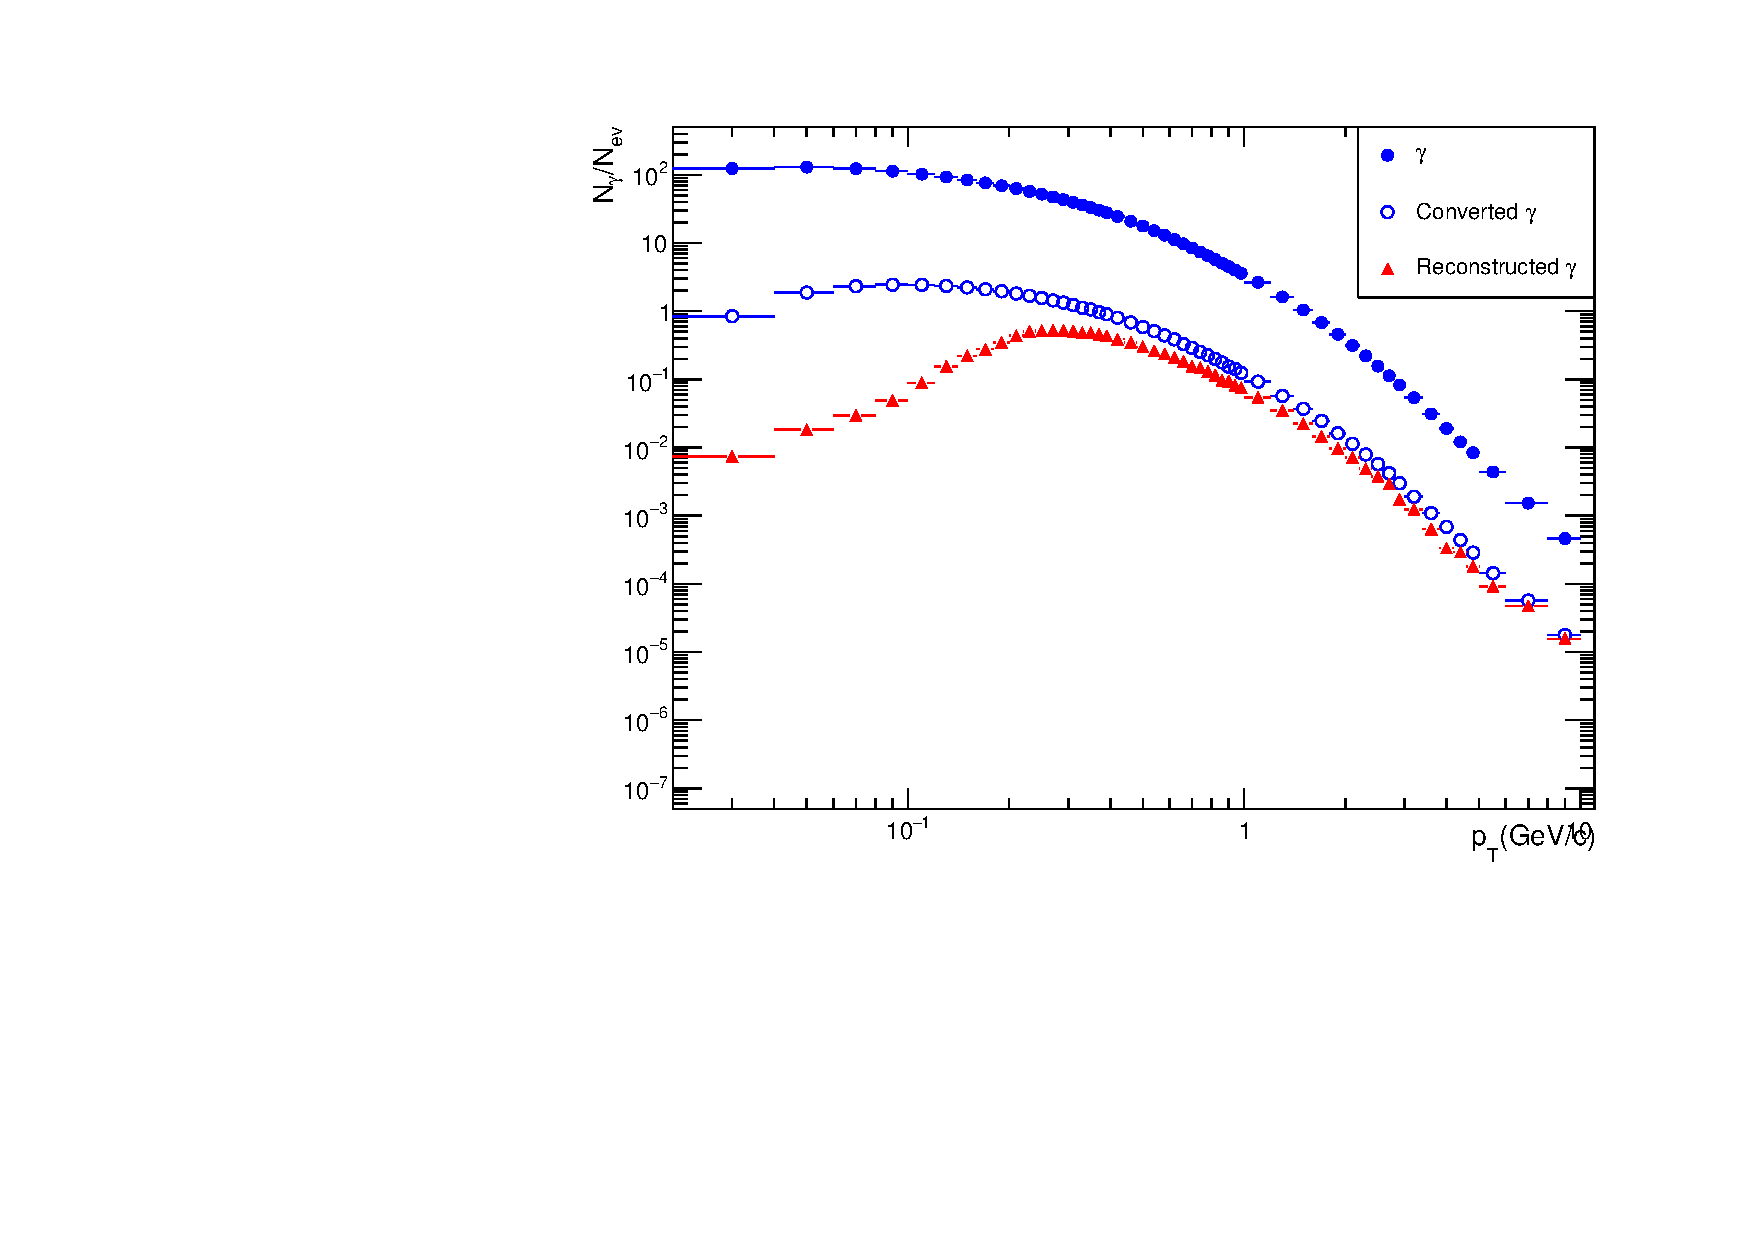
\includegraphics[width=0.38\textwidth]{/Users/marin/alice3/alice3Conversions/anaConv/files220103/PhotonPrimConvRec.pdf}
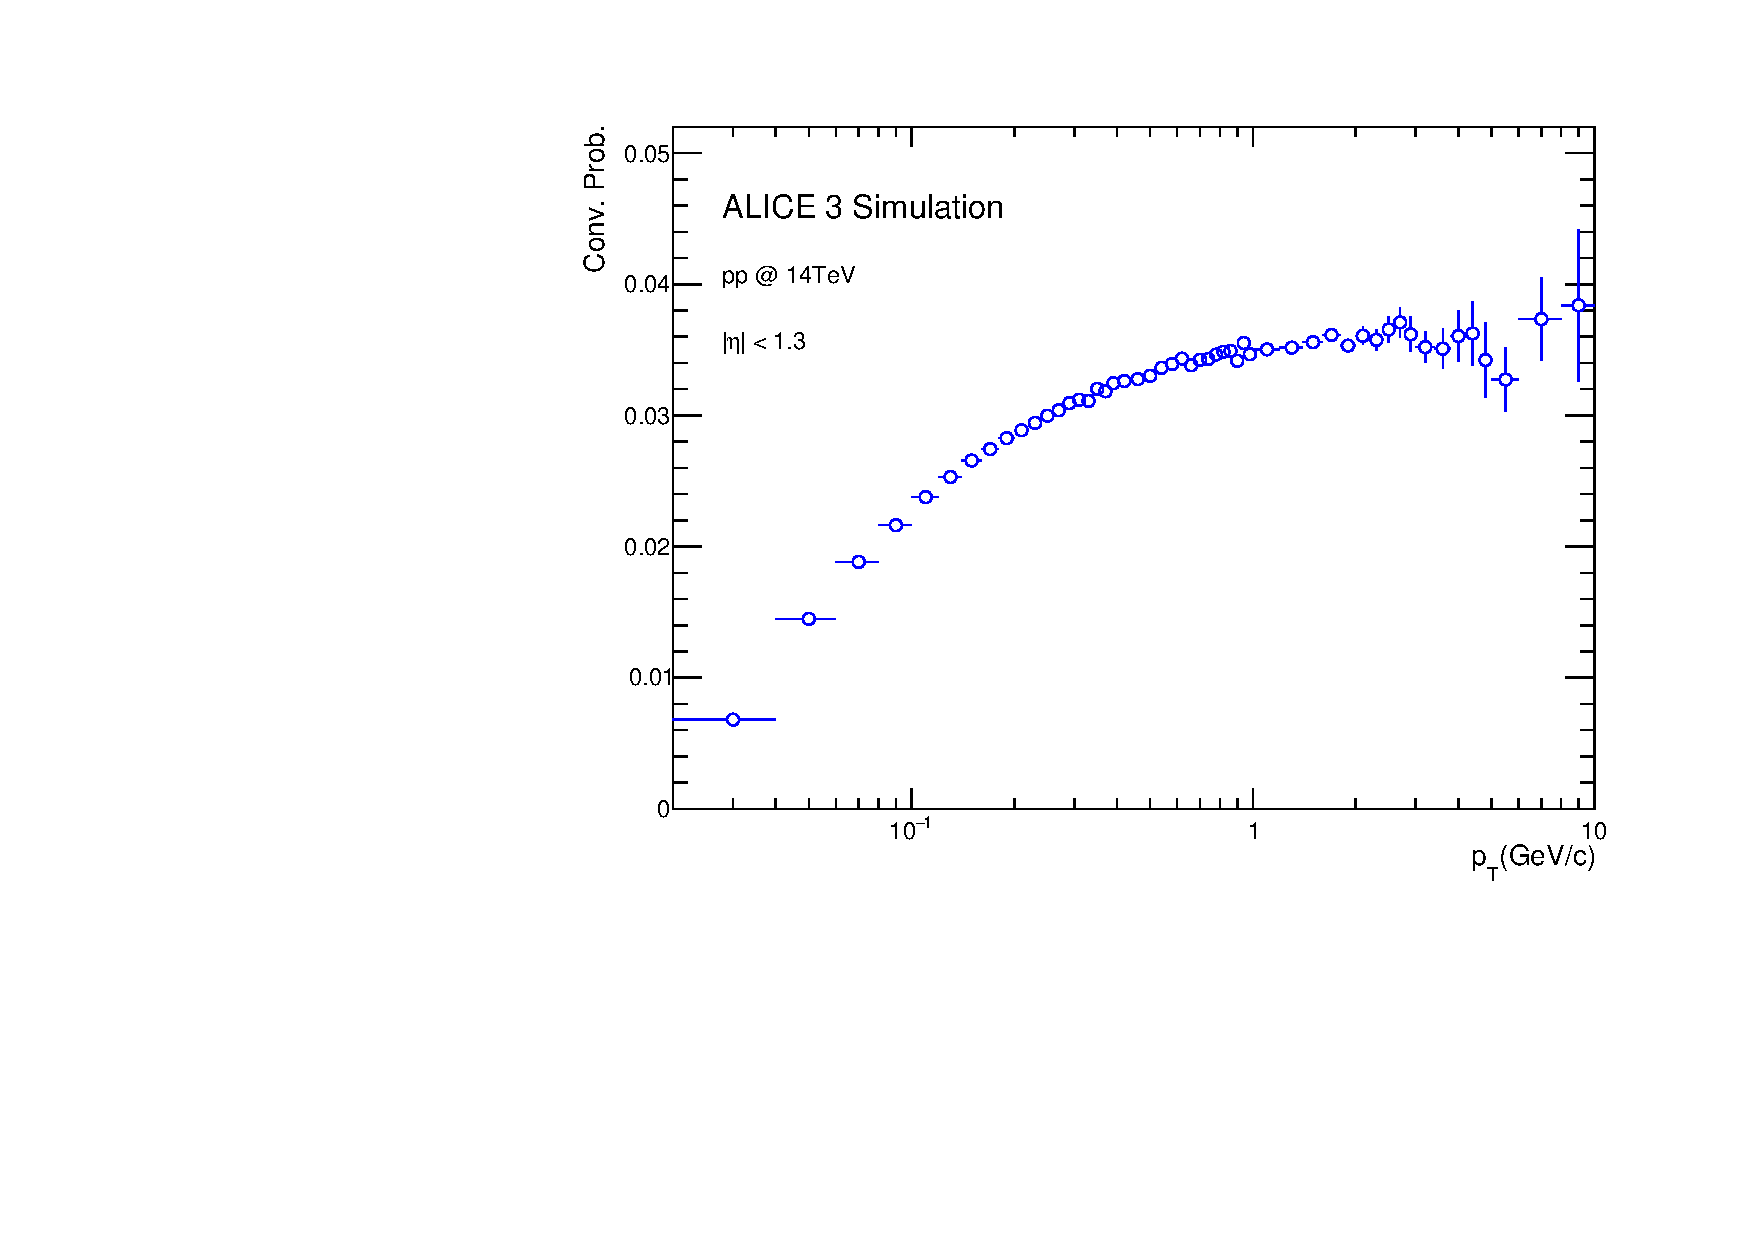
\includegraphics[width=0.38\textwidth]{/Users/marin/alice3/alice3Conversions/anaConv/files220103/PhotonConvProb.pdf}
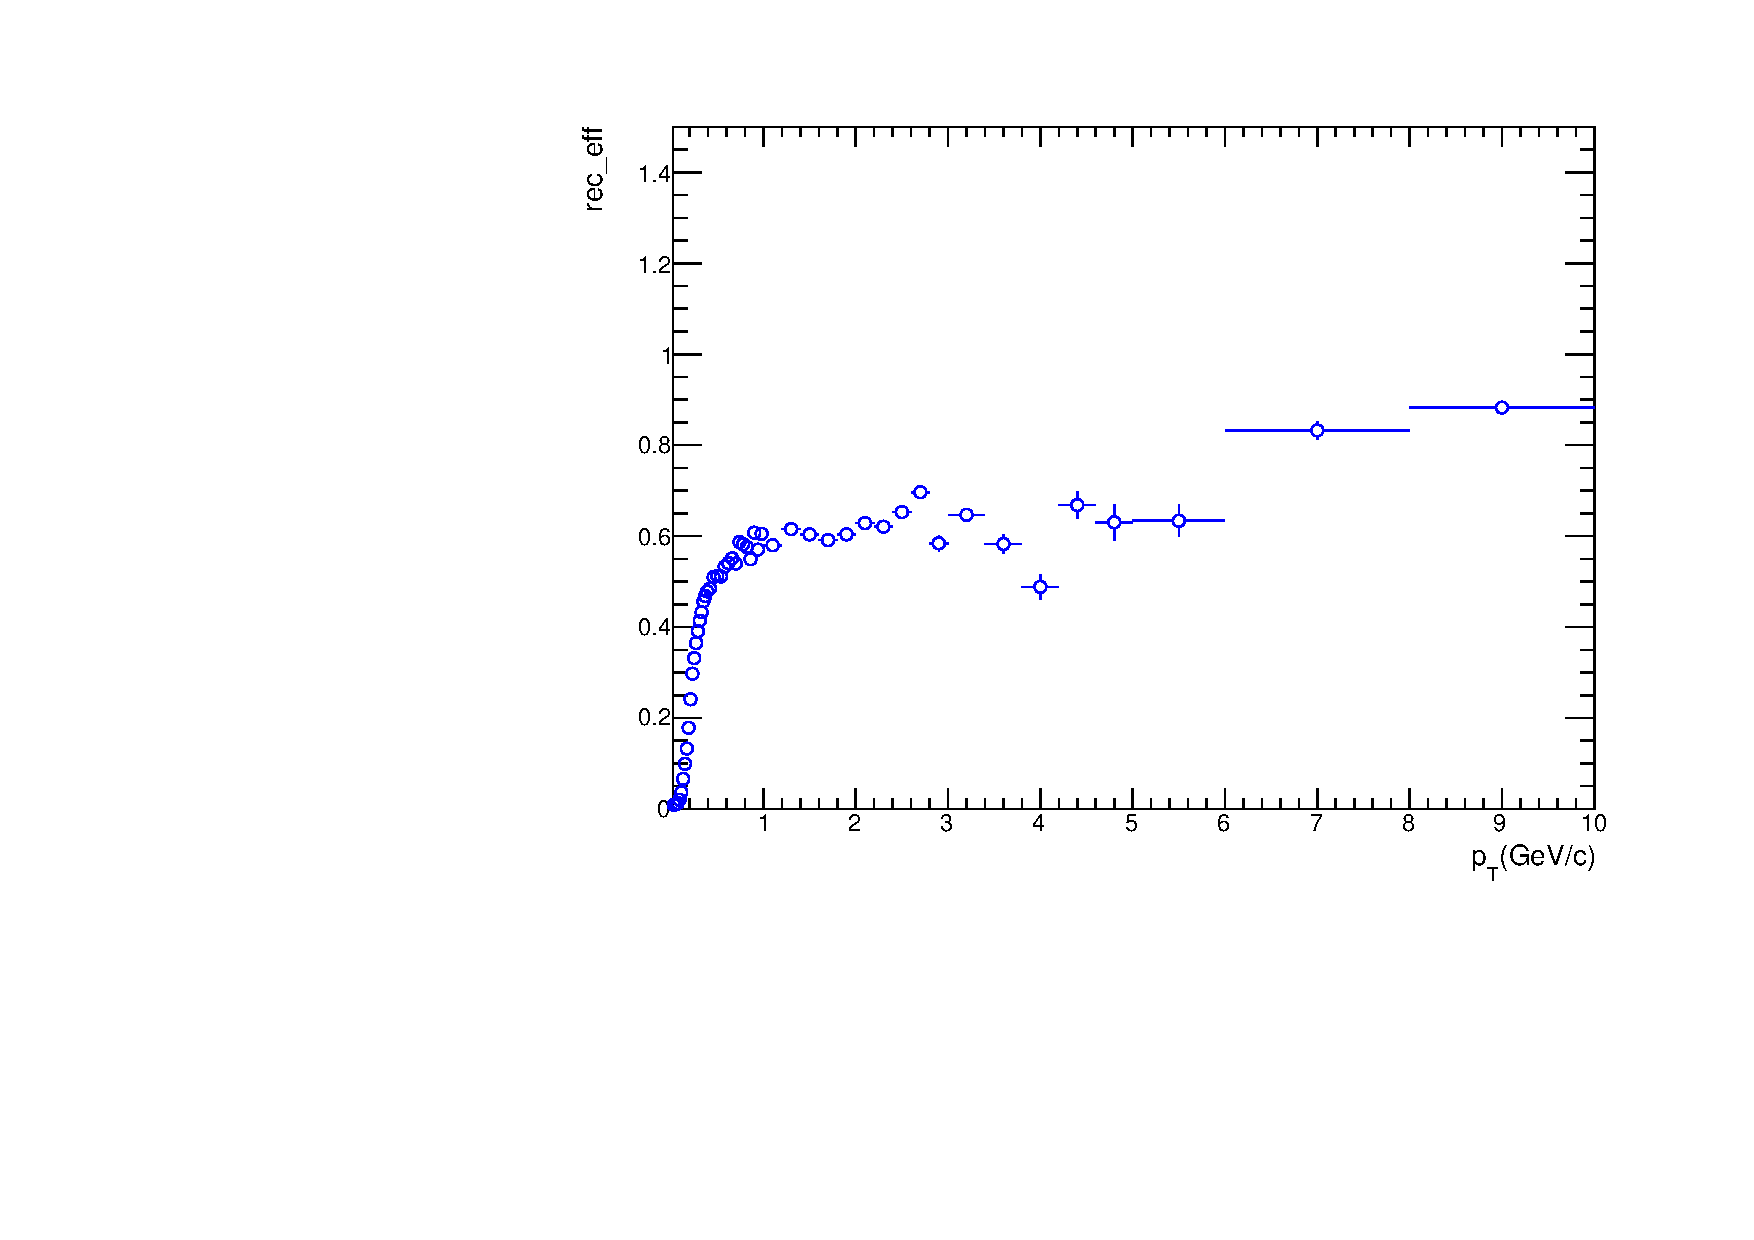
\includegraphics[width=0.38\textwidth]{/Users/marin/alice3/alice3Conversions/anaConv/files220103/PhotonRecEff.pdf}
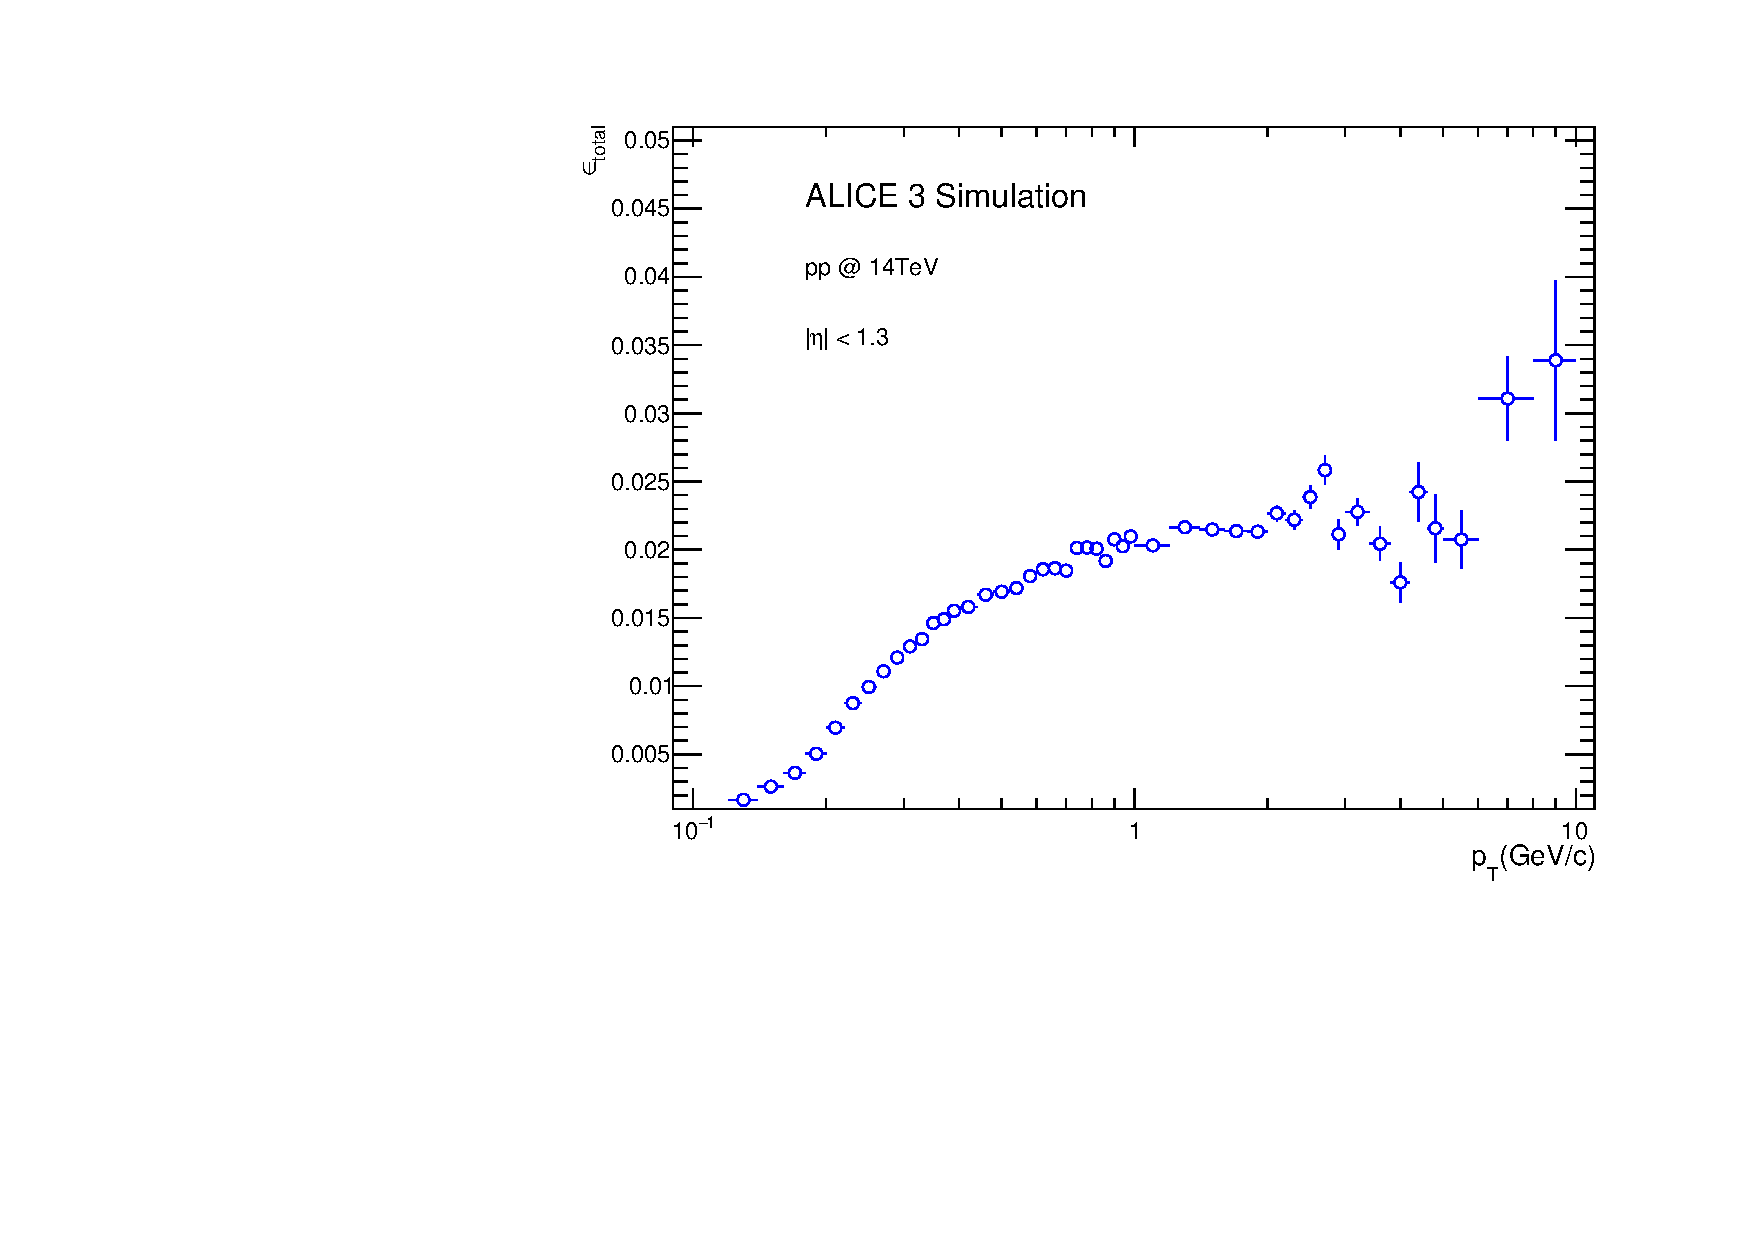
\includegraphics[width=0.38\textwidth]{/Users/marin/alice3/alice3Conversions/anaConv/files220103/totEff.pdf}
\end{frame}

\begin{frame}
\frametitle{Central Barrel: $\gamma$ resolution} 

%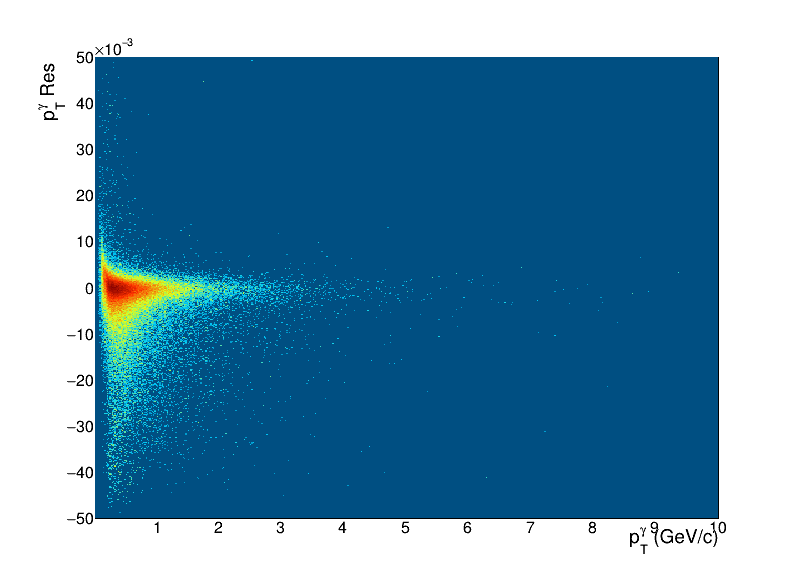
\includegraphics[width=0.38\textwidth]{/Users/marin/alice3/alice3Conversions/anaConv/files220103/PhotonRes.png}

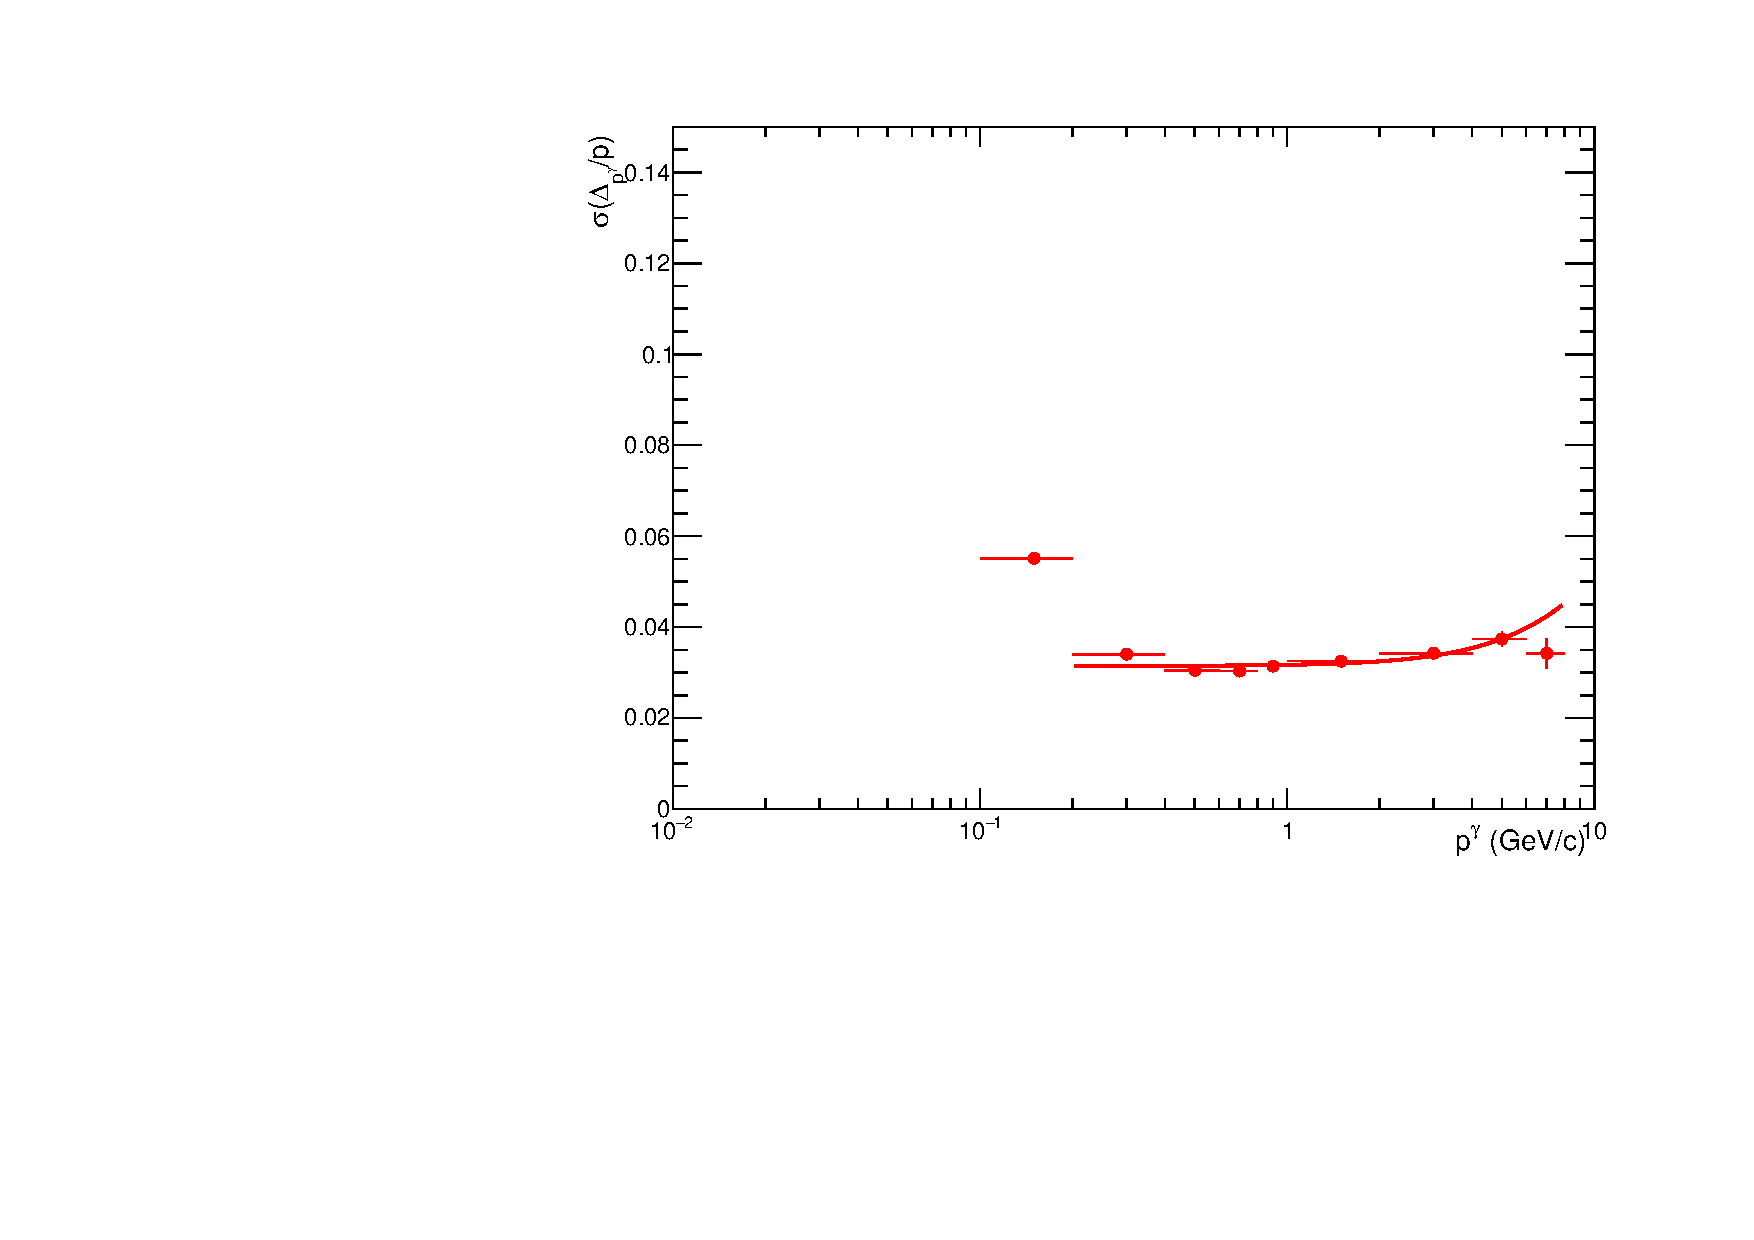
\includegraphics[width=0.38\textwidth]{/Users/marin/alice3/alice3Conversions/anaConv/files220103/PhotonResSigma.pdf}
\end{frame}

\begin{frame}
\frametitle{Forward Barrel: $\gamma$ reconstruction} 

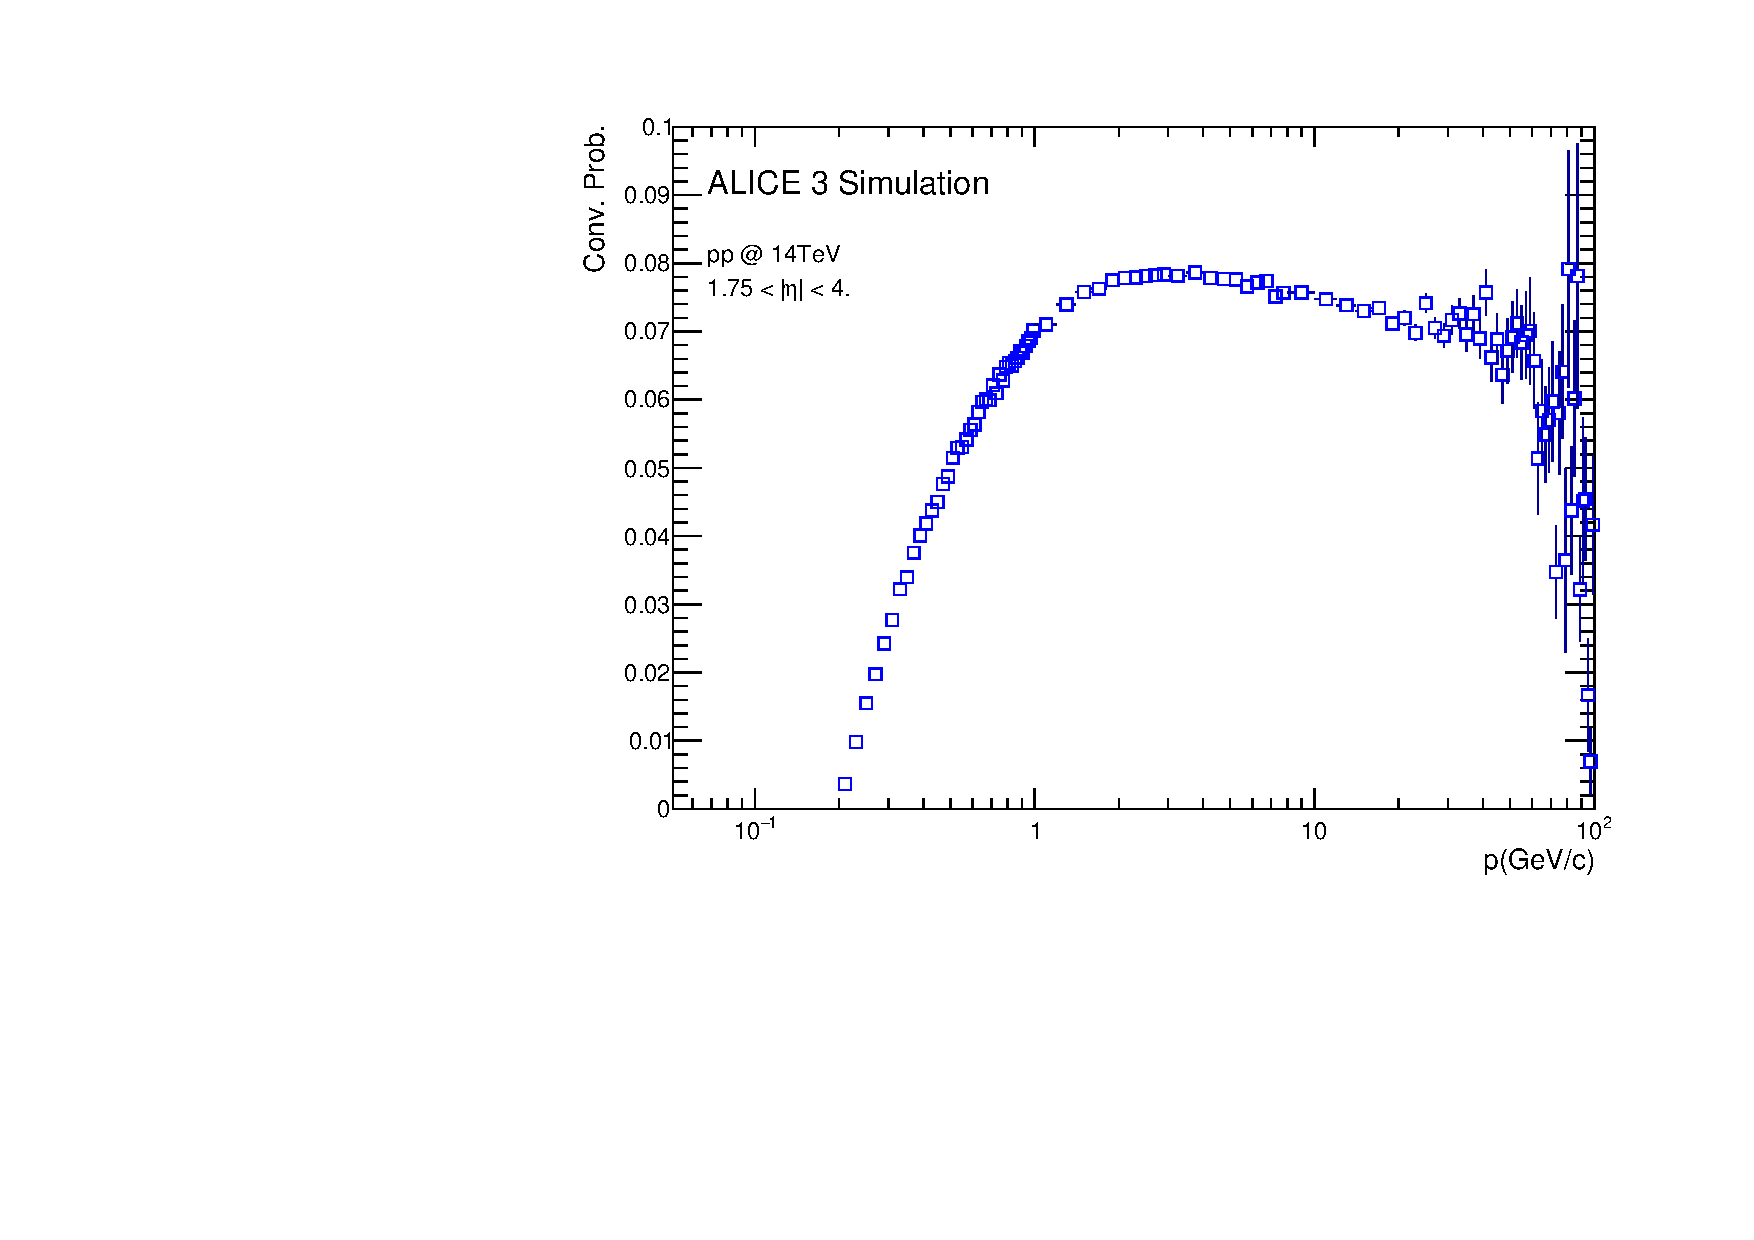
\includegraphics[width=0.4\textwidth]{/Users/marin/alice3/alice3Conversions/anaConv/files220103/PhotonConvProbF.pdf}
\end{frame}

\begin{frame}
\frametitle{Central Barrel: $\chi_{\rm C}$ $\rightarrow$ J/$\psi$ + $\gamma$} 

Delphes Simulation\\


\centering
\includegraphics[width=0.48\textwidth]{/Users/marin/alice3/chic/ChicMassPCM.pdf}
\includegraphics[width=0.48\textwidth]{/Users/marin/alice3/chic/ChicMassPCM_chi1_chi2.pdf}

\end{frame}
\begin{frame}{Delphes simulations used}

{\tiny
For signal :\\
\begin{itemize}
\item $/data2/amarin/productions/ECAL+PCM/delphes/pp\_onia\_X\_2022\_01\_18\_full/$\\
$/home/amarin/alice/Run3Analysisvalidation/codeHF/AnalysisResults\_O2\_PCM\_config21\_Chic1\_Chic2.root$\\

\item $/data2/amarin/productions/ECAL+PCM/delphes/pp\_onia\_X\_2022\_01\_23_full/$\\
$/home/amarin/alice/Run3Analysisvalidation/codeHF/AnalysisResults\_O2\_PCM\_config22\_Chic1\_Chic2.root$
\end{itemize}


For background:
\begin{itemize}
\item PbPb\\
$/home/mmazzill/PbPb\_100K\_inel\_2T\_rmin100\_11102021$\\
$/home/amarin/alice/Run3Analysisvalidation/codeHF/AnalysisResults\_O2\_input\_config16.root$
\item pp\\
$/home/mmazzill/pp14TeV\_inel\_20M\_2T\_rmin100\_geometry\_v1\_11102021$\\
$/home/amarin/alice/Run3Analysisvalidation/codeHF/AnalysisResults\_O2\_input\_config17.root$
\end{itemize}
}
\end{frame}

\begin{frame}
\frametitle{PCM: Signal  estimation} 
\centering

\includegraphics[width=0.85\textwidth]{/Users/marin/alice3/chic/plots/fit_signal_chic_PCM.pdf}\\
%\includegraphics[width=0.48\textwidth]{/Users/marin/alice3/chic/plots/fit_bkg_chic_PCM.pdf}
\end{frame}

\begin{frame}
\frametitle{PCM: Background estimation} 
\centering
%\includegraphics[width=0.48\textwidth]{/Users/marin/alice3/chic/plots/fit_signal_chic_PCM.pdf}\\
\includegraphics[width=0.85\textwidth]{/Users/marin/alice3/chic/plots/fit_bkg_chic_PCM.pdf}
\end{frame}






\begin{frame}
\frametitle{Reconstruction efficiency: PCM and ECAL} 
\includegraphics[width=0.48\textwidth]{/Users/marin/alice3/chic/plots/Efficiency_chic_PCM.pdf}
\includegraphics[width=0.48\textwidth]{/Users/marin/alice3/chic/plots/Efficiency_chic_ECAL.pdf}

\end{frame}


\begin{frame}
\frametitle{Background per event: PCM and ECAL} 

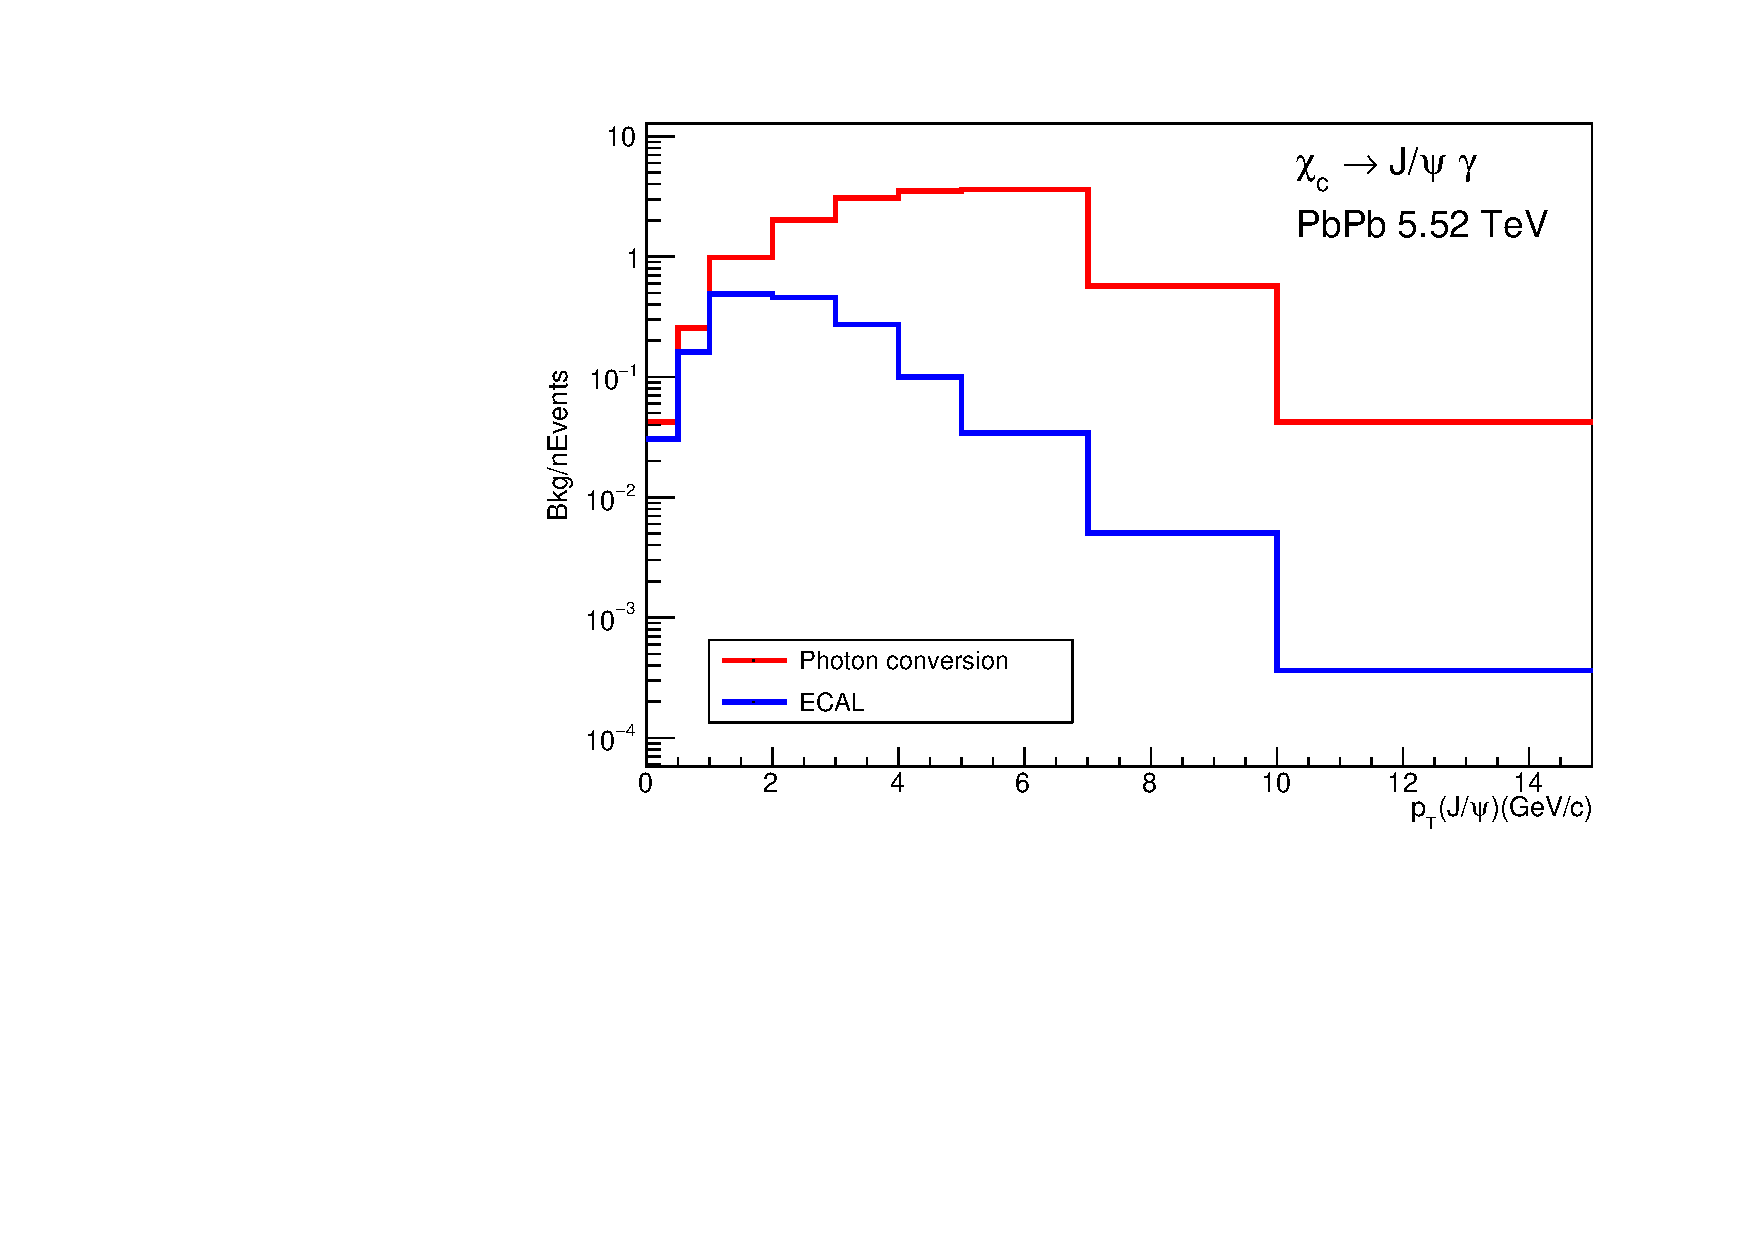
\includegraphics[width=0.48\textwidth]{/Users/marin/alice3/alice3Conversions//presentations/bkgPerEvent_chic_PbPb.pdf}
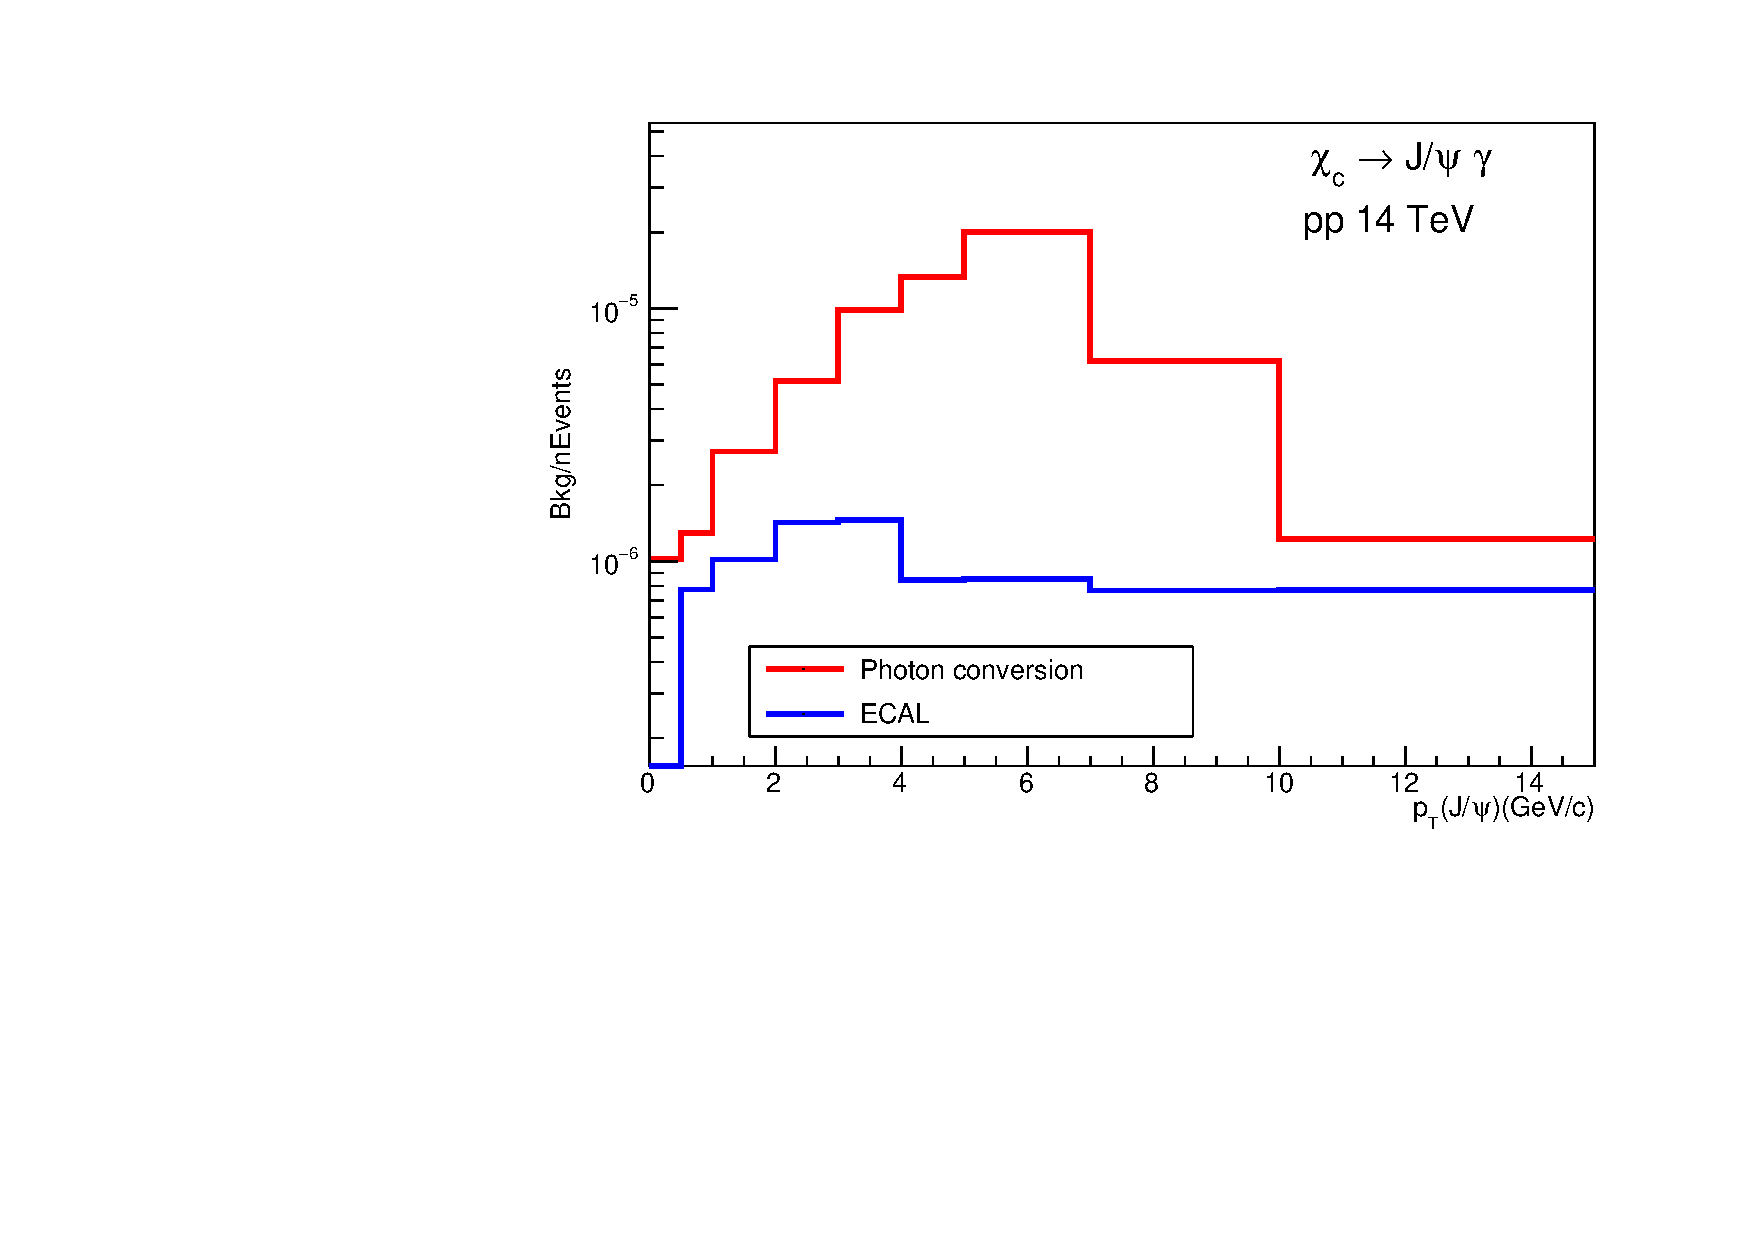
\includegraphics[width=0.48\textwidth]{/Users/marin/alice3/alice3Conversions//presentations/bkgPerEvent_chic_pp.pdf}
\end{frame}


\begin{frame}
\frametitle{Significance in pp: PCM and ECAL} 
\includegraphics[width=0.42\textwidth]{/Users/marin/alice3/chic/plots/Chi_c_PCM_pp14p0_absy1p44_results.pdf}
\includegraphics[width=0.42\textwidth]{/Users/marin/alice3/chic/plots/Chi_c_pp14p0_absy1p44_results.pdf}

Significance calculated as sum of $\chi_{\rm C1}$ and $\chi_{\rm C2}$\\
Combination of ECAL and PCM measurements will improve the significance

\end{frame}

\begin{frame}
\frametitle{Significance in PbPb: PCM and ECAL} 
\includegraphics[width=0.42\textwidth]{/Users/marin/alice3/chic/plots/Chi_c_PCM_PbPb5p52_absy1p44_results.pdf}
\includegraphics[width=0.42\textwidth]{/Users/marin/alice3/chic/plots/Chi_c_PbPb5p52_absy1p44_results.pdf}

Significance calculated as sum of $\chi_{\rm C1}$ and $\chi_{\rm C2}$\\
\end{frame}

\begin{frame}{Proposed additions to the LOI}

{\tiny
569 .... These states could also\\
 570 be separated by reconstructing the photons through their conversion in the material, benefiting\\
 571 from the good momentum resolution for charged particles.\\
\textcolor{blue}{Indeed, an initial simulation effort, described in Fig~\ref{}... in section 'performance', demonstrates very good resolution\\
 in the measurement with the conversion method of the $\chi_c$ states as produced in pp collisions.}\\
}
\vspace{1cm}
\includegraphics[width=0.4\textwidth]{/Users/marin/alice3/chic/ChicMassPCM_chi1_chi2.pdf}

Place figure in section 3.2.2.2\\
\end{frame}

\begin{frame}{Proposed additions to the LOI}

%\vspace{1cm}
{\tiny
Section 3.3.2.2 $\chi_c$ and $\chi_b$ states\\
2519 As discussed in Section 2.2.1, a comprehensive study of charmonium states in heavy-ion colli-  \\
2520 sions should include a characterization of P-wave states such as $\chi_c$ and $\chi_b$. With ALICE 3, this  \\
2521 can be achieved by reconstructing decays in the $\chi_c$J $\rightarrow$J/$\psi$ + $\gamma$ decay channel using the muon  \\
2522 identifier to reconstruct J/$\psi$ and the electromagnetic calorimeter to detect decay photons (see  \\
Section 4.5.1) \textcolor{blue}{or the photon conversion method (see Fig.~\ref{}).}\\


2524 The reconstruction of the $\chi_c$ candidates starts with the reconstruction of the J/$\psi$ candidates fol \\
2525 lowing the strategy discussed in Section 3.3.2.1. Each selected J/$\psi$ candidate is then combined\\
2526 with the available photons detected in the same event. In order to select a clean sample of $\chi_c$\\
2527 candidates and to reduce the combinatorial background, the cuts reported for the J/$\psi$ analysis\\
2528 are applied, combined with a 2$\sigma$ cut on the invariant mass of the J/$\psi$ candidate and a lower cut\\
2529 on the photon energy E$\gamma$ $>$ 400 MeV {\textcolor{blue}{in case of the ECAL}}. Figure 47 shows the significance of the $\chi_c$ measurement\\
2530 (sum of the $\chi_{c1}$ and $\chi_{c2}$ signals) corresponding to the currently implemented kinematic cuts, as a\\
2531 function of transverse momentum in pp collisions at $\sqrt{s}$ = 14 TeV (Lint = 18fb$^{-1}$) and in Pb-Pb\\
2532 collisions at $\sqrt{s_{NN}} $= 5:5 TeV (Lint = 35nb$^{-1}$) {\textcolor{blue}{for the ECAL and PCM methods}}. A dedicated optimization of the cuts is currently\\
2533 undergoing, involving machine learning techniques based on boosted decision trees. \\
{\textcolor{blue}{Special runs with a converter may be needed to increase the significance for the PCM measurements in HIC.}}\\
}

\vspace{1cm}

\textcolor{blue}{\small Create a Figure 47, where the significance of both methods (ECAL and PCM) is shown simultaneously}
\end{frame}

%\begin{frame}{Proposed additions to the LOI}

%\includegraphics[width=0.42\textwidth]{/Users/marin/alice3/chic/plots/Chi_c_PCM_pp14p0_absy1p44_results.pdf}

%\end{frame}

\end{document}

\begin{frame}
\frametitle{Significance in pp: PCM and ECAL} 
\includegraphics[width=0.32\textwidth]{/Users/marin/alice3/chic/plots/Chi_c_PbPb5p52_absy1p44_results.pdf}
\includegraphics[width=0.32\textwidth]{/Users/marin/alice3/chic/plots/Chi_c_pp14p0_absy1p44_results.pdf}
\includegraphics[width=0.32\textwidth]{/Users/marin/alice3/chic/plots/Chi_c_PCM_pp14p0_absy1p44_results.pdf}
\includegraphics[width=0.32\textwidth]{/Users/marin/alice3/chic/plots/Chi_c_PCM_PbPb5p52_absy1p44_results.pdf}
\end{frame}




